\chapter{Especificaciones del robot delta seleccionado}\label{CAP5}
En este capítulo se proponen los parámetros dimensionales y físicos para las simulaciones del robot delta. Estos valores generalmente se obtienen de la optimización dimensional de las piezas por energía y por los límites de un espacio de trabajo determinado para una aplicación específica, sin embargo no es el objetivo de esta tesis, por lo que se extraen los valores del prototipo del robot delta de la tesis \cite{upm378}. Los datos se ingresan al archivo $pd\_tm1\_adams.py$.


    \begingroup
        \renewcommand{\arraystretch}{1.5}
        \begin{table}[H]
        \centering
        \begin{tabular}{c c{4cm} c}
           \hline
           \textbf{Parametro}  & \multicolumn{1}{c}{\textbf{Descripción}} & Valor \\\hline\hline
            $L_1$  & Longitud de un brazo           & 620 [mm]                        \\\hline
            $L_2$  & Longitud de un antebrazo       & 880 [mm]                         \\\hline
            $R_A$  & Radio de la base fija           & 210 [mm]                         \\\hline
            $R_B$  & Radio de la plataforma móvil    & 50 [mm]                         \\\hline
            $m_1$  & Masa de un brazo                & 2.213 [kg]                         \\\hline
            $m_2$  & Masa de una varilla del antebrazo  & 0.6575 [kg]                         \\\hline
            $m_p$  & Masa de la plataforma móvil     & 0.510 [kg]                         \\\hline
            $m_{playload}$  & Masa de carga que es trasladada por el efector & 0 [kg]           \\\hline
            $m_{elbow}$  & Masa de juntas que conectas los brazos con los antebrazos  & 0 [kg]  \\\hline
            $I_m$  & Inercia de los actuadores           &   0 [kg*m^2]     \\\hline
            $r_{mass}$  & Relación masas antebrazo           & 0.5        \\\hline
            $g$  & Gravedad           & 9.81  [m/s^2]                      \\\hline 
        \end{tabular}
        \caption{Parámetros necesarios para la simulación del robot delta en esta tesis}
        \label{tab:cap5_tabla_1}
    \end{table}
    \endgroup
    
    \newpage
    
     La simplificación del robot delta se presenta en la figura \eqref{fig:cap5_1}.
    
    \begin{figure}[htb]
        \centering
        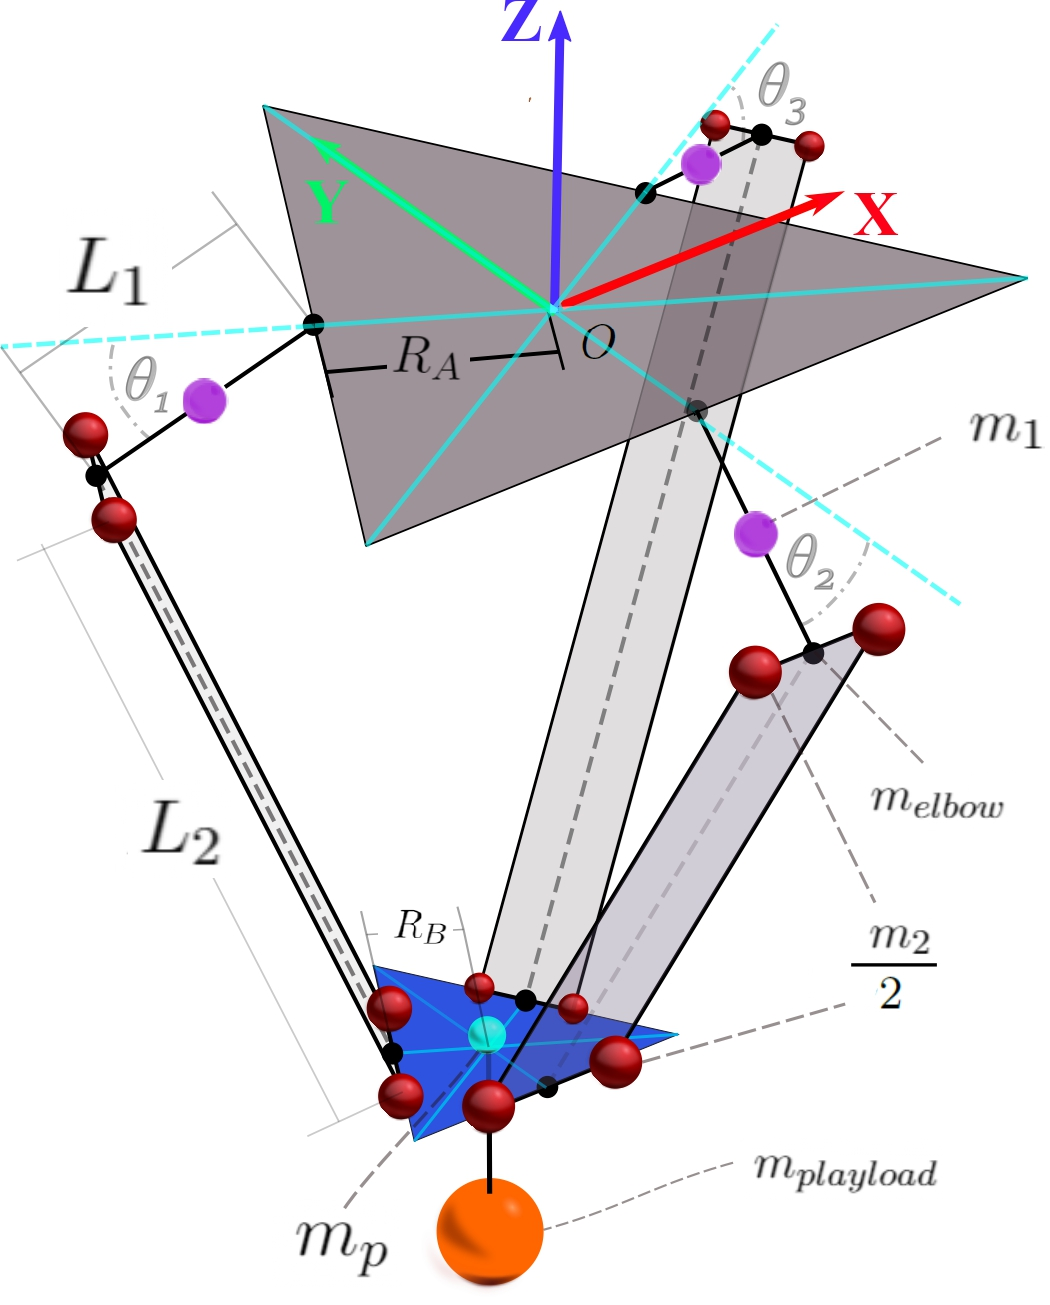
\includegraphics[width=0.87\linewidth]{Main/Chapter5/Images5/DIBUJO55.jpg}
        \caption{Representación gráfica, marco de referencia, dimensiones, masas y orden de ángulos del robot delta a simular.}
        \label{fig:cap5_1}
    \end{figure}
    
    
    